\documentclass{article}
\usepackage{lmodern}
\usepackage{amsmath}
\usepackage{amssymb}
\usepackage[T1]{fontenc}
\usepackage{listings}
\usepackage{fancyhdr}
\usepackage{hyperref}
\usepackage{pdfpages}

\pagestyle{fancy}
\lhead{Anirudhan J Rajagopalan - ajr619 - N18824115} % chktex 8

\begin{document}

\title{Foundations of Machine Learning --- Homework Assignment 1}
\date{October 11, 2015}
\author{Anirudhan J Rajagopalan\\ N18824115\\ ajr619}

\maketitle

\newpage

\section*{C. Support Vector Machines}
\subsection*{1}
Installed the software from\cite{libsvm}.  The installed version of software is also checked into github at\cite{githuburl}. 
\subsection*{2}

\noindent See the following command:
\begin{lstlisting}[language=bash]
  $ ./svm-scale -s splice_noise_train.txt.range \ 
  > splice_noise_train.txt > splice_noise_train.txt.scale
  $ ./svm-scale -r splice_noise_train.txt.range \
  > splice_noise_test.txt > splice_noise_test.txt.scale
\end{lstlisting}

\subsection*{3}
Run training and test script\cite{cvscript} by editing the KERNEL\_DEGREE parameter for each value of d = 1, 3, 5.
\begin{lstlisting}
  $ python cross_validation.py > deg1.out # KERNEL_DEGREE = 1
  $ python cross_validation.py > deg3.out # KERNEL_DEGREE = 3
  $ python cross_validation.py > deg5.out # KERNEL_DEGREE = 5
\end{lstlisting}

Filter the parameter and accuracy information from the run logs (deg1.out, deg3.out and deg5.out) by the command below.
\begin{lstlisting}
  $ cat deg1.out | grep OUR | cut -d' ' \
  > -f2,3,4,5,6 > deg1.out.filtered
  $ cat deg3.out | grep OUR | cut -d' ' \
  > -f2,3,4,5,6 > deg3.out.filtered
  $ cat deg5.out | grep OUR | cut -d' ' \
  > -f2,3,4,5,6 > deg5.out.filtered
\end{lstlisting}

Use plotter.py\cite{plotterpy} to create plots from the output values for KERNEL\_DEGREE values 1, 3, 5.  The output will be saved as deg1.pdf, deg3.pdf and deg5.pdf.  All the three plots are embedded below one after the other.
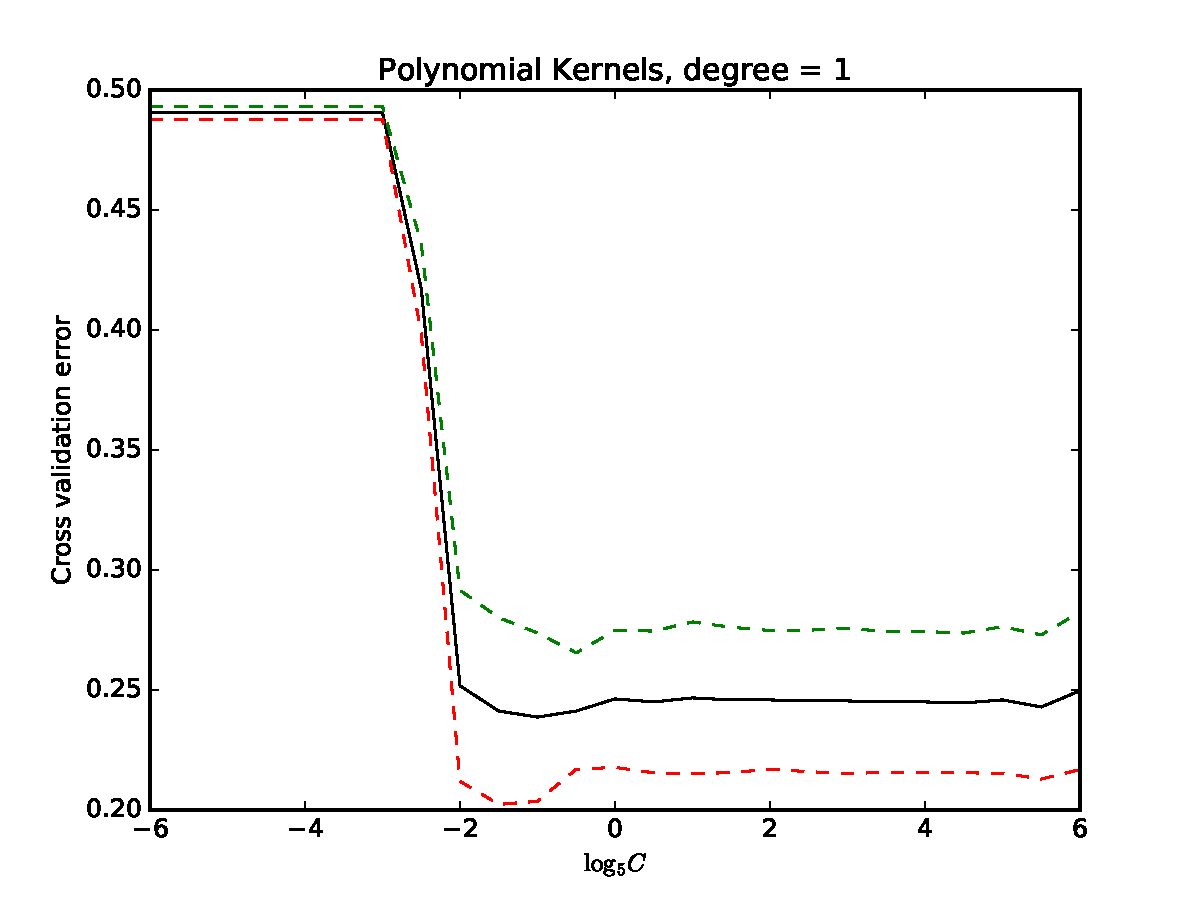
\includepdf[pages={1},lastpage={1}]{libsvm-3.20/tools/deg1.pdf}
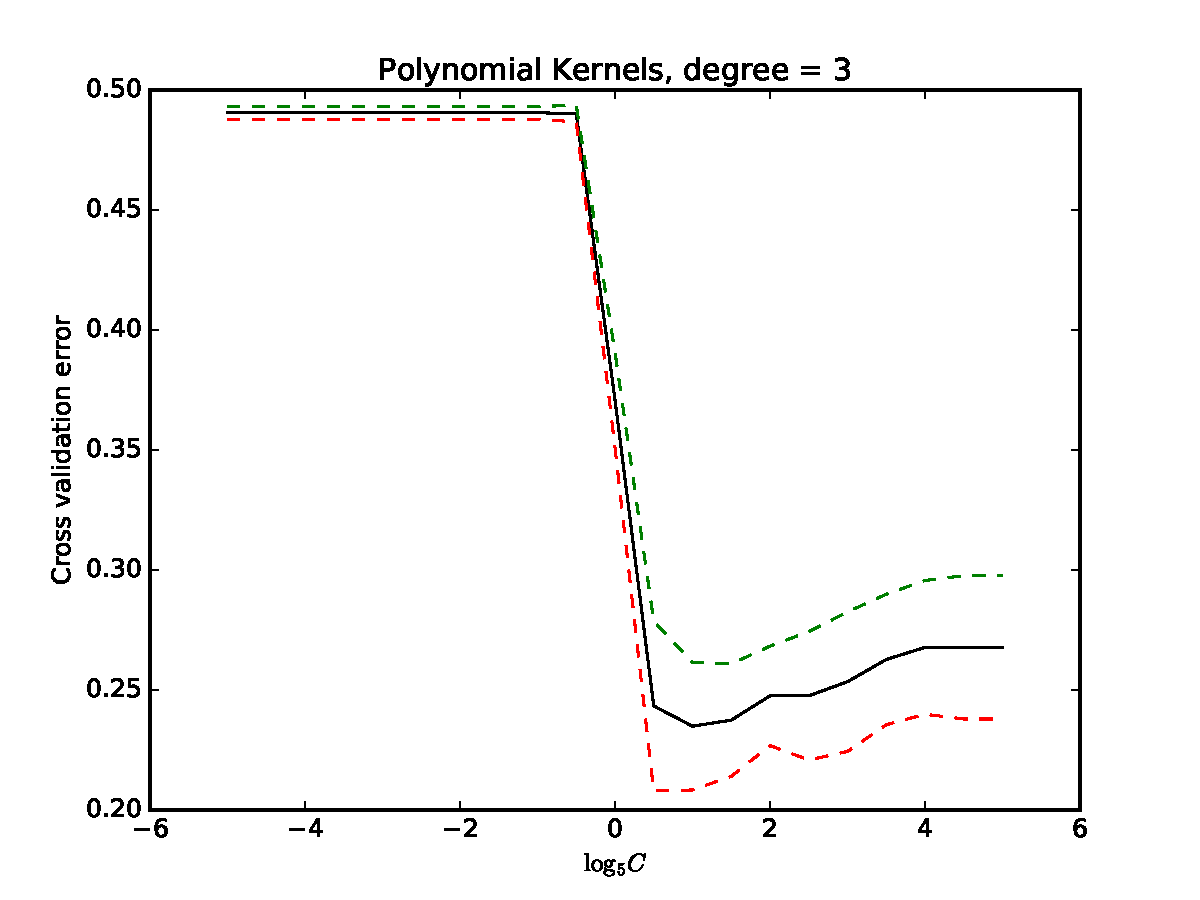
\includepdf[pages={1},lastpage={1}]{libsvm-3.20/tools/deg3.pdf}
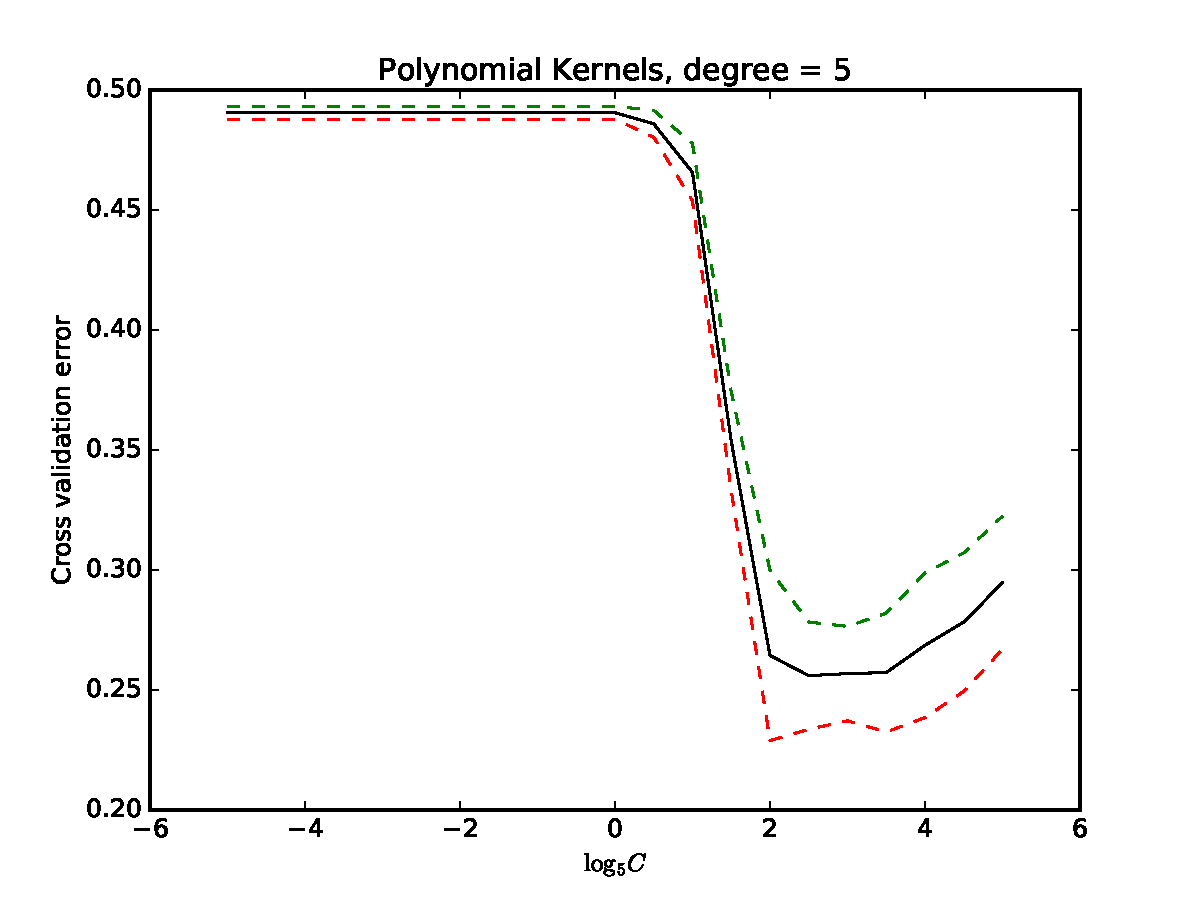
\includepdf[pages={1},lastpage={1}]{libsvm-3.20/tools/deg5.pdf}
\subsection*{4}
\subsection*{5}
\subsection*{6}

\section*{D. Kernels}
\subsection*{1}
\begin{description}
  \item{Given:} Kernel, K is defined by \(K(x,y) = \sum_{i=1}^{N} \cos^{n} (x_{i}^{2} - y_{i}^{2} )\) for all \((X, Y) \in \mathbb{R}^{N} \times \mathbb{R}^{N} \) 
  \item{Solution:}  We know that
    \begin{equation}
      \cos (x_{i}^{2} - y_{i}^{2}) = \sin (x_{i}^{2}).\sin (y_{i}^{2}) + \cos (x_{i}^{2}).\cos (y_{i}^{2})
    \end{equation}
    This can be written as a dot product of two vectors 
    \begin{align}
    \phi(x_{i}) = \begin{bmatrix} \cos (x_{i}^{2}) \\ \sin (x_{i}^{2}) \end{bmatrix} && \mathrm{and} &&
    \phi(y_{i}) = \begin{bmatrix} \cos (y_{i}^{2}) \\ \sin (y_{i}^{2}) \end{bmatrix}
    \end{align}

    We know that if K can be written as \( \langle \phi(x_{i}), \phi(y_{i}) \rangle \), then it is a PDS@.

    Also, \( \langle \phi(x_{i}), \phi(y_{i}) \rangle \) is a scalar.  When a scalar is raised to a positive power (n in our case) and summed with N other positive scalar, we get a positive scalar as our answer.  Hence
    \begin{equation*}
      K(x,y) = \sum_{i=1}^{N} \cos^{n} (x_{i}^{2} - y_{i}^{2} ) \mathrm{is PDS.}
    \end{equation*}
\end{description}

\begin{thebibliography}{1}
  \bibitem{githuburl} \url{http://git.io/v80yn}
  \bibitem{libsvm} \url{http://www.csie.ntu.edu.tw/~cjlin/libsvm/}
  \bibitem{cvscript} \url{http://git.io/v80yY}
  \bibitem{plotterpy} \url{http://git.io/v80yk}
\end{thebibliography}

\end{document}
